\chapter[Anexos]{Anexos}
\label{chap:anexos}
\addcontentsline{toc}{chapter}{Anexos}


\begin{tcolorbox}[colback=gray!5!white, colframe=gray!60!black, title=Anexo A \- Sesión de captura del conjunto de datos]
	En este anexo se presenta una fotografía del proceso de captura de las señas dinámicas del
	\Acrshort{lesho}. El script de captura, desarrollado en Python con OpenCV, guía a la persona
	que graba mostrando en pantalla la seña que corresponde grabar, el número de repetición
	actual y una retroalimentación en tiempo real de la detección de MediaPipe (mano y cuerpo
	detectados), como se observa en la interfaz de la \autoref{fig:anexo-captura-dinamica}.
\end{tcolorbox}

\begin{figure}[H]
    \centering
    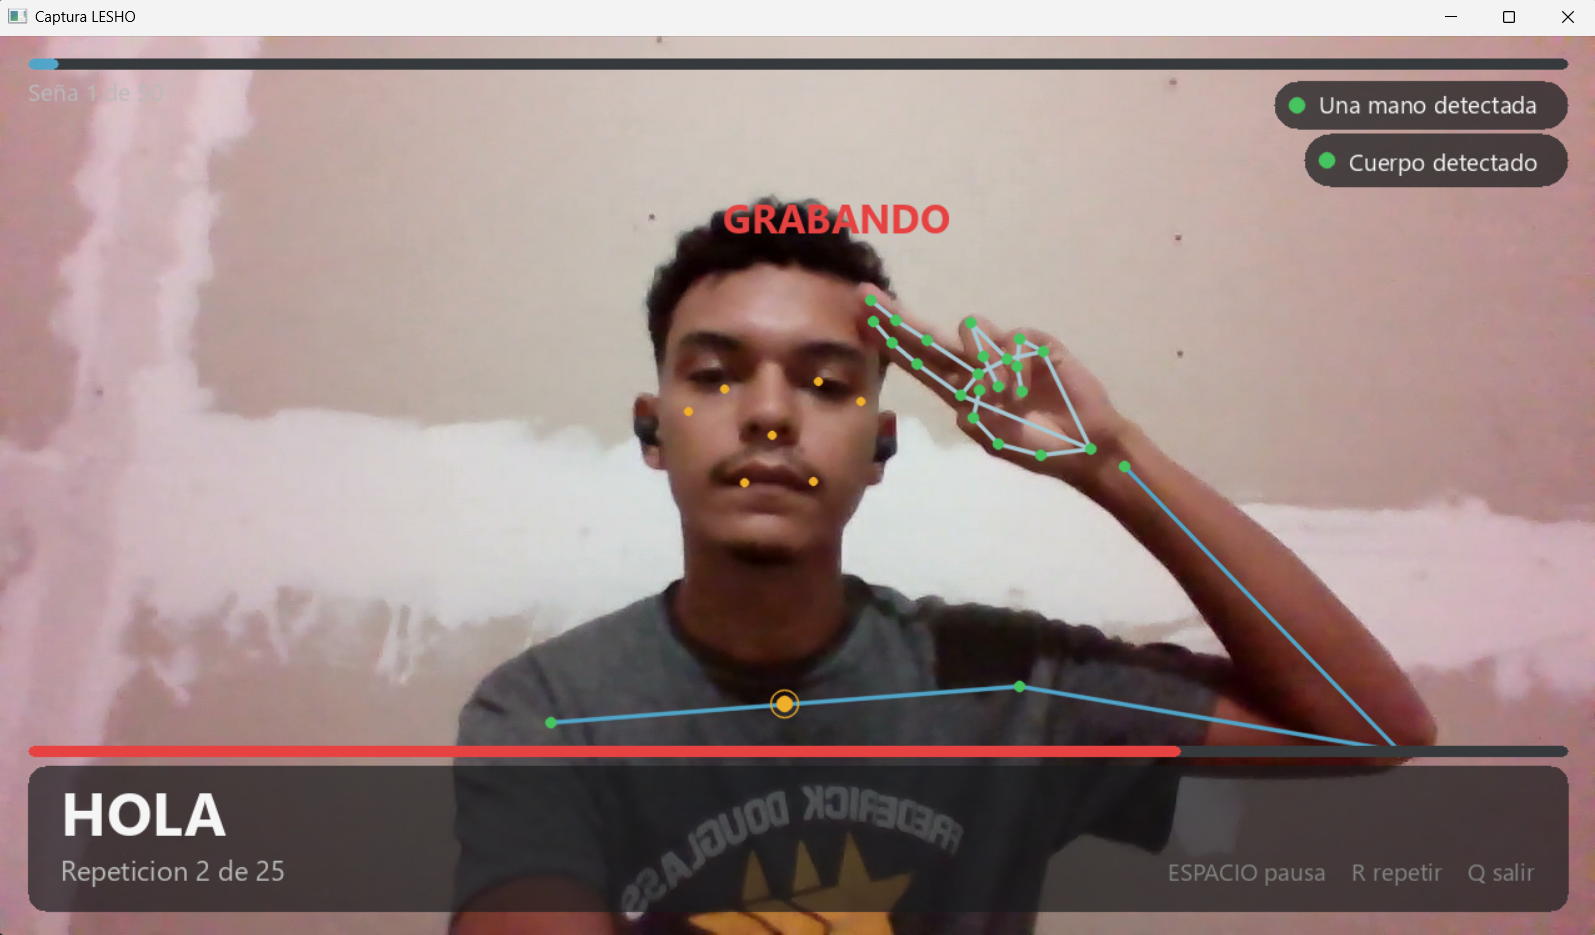
\includegraphics[width=0.8\textwidth]{Figures/Anexos/captura_dinamica.png}
    \caption[Interfaz del script de captura durante la grabación de la seña HOLA]{Interfaz del script de captura durante la grabación de la seña HOLA, con retroalimentación en tiempo real de los landmarks de la mano y del cuerpo detectados por MediaPipe. Fuente: Elaboración propia.}
    \label{fig:anexo-captura-dinamica}
\end{figure}

\clearpage

\begin{tcolorbox}[colback=gray!5!white, colframe=gray!60!black, title=Anexo B \- Fragmento de código para la normalización de landmarks]
	En este anexo se presenta un fragmento de código real del pipeline de entrenamiento,
	correspondiente a la normalización de los landmarks de una mano respecto a la muñeca. Esta
	normalización es la base tanto del Modelo A como del Modelo B, y hace que la representación
	de una seña no dependa de en qué parte del cuadro de la cámara se encuentre la mano.
\end{tcolorbox}

\begin{listing}[H]
    \caption[Fragmento de código en Python para la normalización de landmarks respecto a la muñeca]{Fragmento de código en Python para la normalización de landmarks respecto a la muñeca (\texttt{training/comun/normalizacion.py})}
    \label{cod:anexo-normalizacion}
    \begin{minted}{python}
def normalizar_respecto_muneca(landmarks_crudos) -> list[float]:
    if len(landmarks_crudos) != NUM_LANDMARKS:
        raise ValueError(
            f"Se esperaban {NUM_LANDMARKS} landmarks, "
            f"se recibieron {len(landmarks_crudos)}."
        )

    muneca = landmarks_crudos[INDICE_MUNECA]
    origen_x, origen_y, origen_z = muneca[0], muneca[1], muneca[2]

    vector: list[float] = []
    for punto in landmarks_crudos:
        vector.append(float(punto[0]) - float(origen_x))
        vector.append(float(punto[1]) - float(origen_y))
        vector.append(float(punto[2]) - float(origen_z))

    return vector
    \end{minted}
\end{listing}

\clearpage

\begin{tcolorbox}[colback=gray!5!white, colframe=gray!60!black, title=Anexo C \- Equipo utilizado]
	En este anexo se detalla el equipo utilizado durante el desarrollo del proyecto: la
	computadora empleada para el entrenamiento de los modelos y el teléfono utilizado para las
	pruebas de la aplicación.
\end{tcolorbox}

\begin{itemize}
	\item \textbf{Computadora de entrenamiento:} HP Victus 15, procesador AMD, tarjeta gráfica
	dedicada AMD Radeon RX 6550M (4 GB de memoria de video), 16 GB de memoria RAM y 1 TB de
	almacenamiento.
	\item \textbf{Teléfono de prueba:} Samsung Galaxy A13 (modelo SM-A135M), Android 14,
	arquitectura de 32 bits (armeabi-v7a), utilizado para validar la aplicación en un
	dispositivo de gama baja representativo del contexto hondureño.
\end{itemize}
